\documentclass[12pt, a4paper]{article}

\usepackage[utf8]{inputenc}
% Limit the page margin to only 1 inch.
\usepackage[margin=1in]{geometry}

%Imports biblatex package
\usepackage[
backend=biber,
style=alphabetic
]{biblatex}
\addbibresource{../../algs4e.bib}

% Enables the `align' environment.
\usepackage{amsmath}
% Provides useful environments, such as:
% - \begin{proof} ...\end{proof}
\usepackage{amsthm}
\usepackage[most]{tcolorbox}

\newtheorem*{proposition}{Proposition}

% Enables using \mathbb{}, for example \mathbb{N} for the set of natural numbers.
\usepackage{amssymb}

% Allows using letters in enumerate list environment. Use, for example:
%\begin{enumerate}[label=(\alph*)]
% ...
%\end{enumerate}
\usepackage[inline]{enumitem}

% Enable importing external graphic files and provides useful commannds, like \graphicspath{}
\usepackage{graphicx}
% Images are located in a directory called images in the current directory.
\graphicspath{{./images/}}

% Make links look better by default.
% See: https://tex.stackexchange.com/questions/823/remove-ugly-borders-around-clickable-cross-references-and-hyperlinks
\usepackage[hidelinks]{hyperref}
\usepackage{xcolor}
\hypersetup{
	colorlinks,
	linkcolor={red!50!black},
	citecolor={blue!50!black},
	urlcolor={blue!80!black}
}


% Code Listings. Source:
% https://stackoverflow.com/questions/3175105/inserting-code-in-this-latex-document-with-indentation
\usepackage{listings}
\usepackage{color}

\definecolor{dkgreen}{rgb}{0,0.6,0}
\definecolor{gray}{rgb}{0.5,0.5,0.5}
\definecolor{mauve}{rgb}{0.58,0,0.82}

\lstset{frame=tb,
	language=Java,
	aboveskip=3mm,
	belowskip=3mm,
	showstringspaces=false,
	columns=flexible,
	basicstyle={\small\ttfamily},
	numbers=none,
	numberstyle=\tiny\color{gray},
	keywordstyle=\color{blue},
	commentstyle=\color{dkgreen},
	stringstyle=\color{mauve},
	breaklines=true,
	breakatwhitespace=true,
	tabsize=3
}

\newcommand{\prob}{\text{P}}
%\newcommand{\complement}{\mathsf{c}}

% Define an environment called "ex" (for Exercise) so that I can do: \begin{ex}{1.5}...\end{ex}
\newenvironment{ex}[2][Exercise]
{\par\medskip\noindent \textbf{#1 #2.}}
{\medskip}

% Define a solution environment, similar to ex (exercise) environment.
\newenvironment{sol}[1][Solution]
{\par\medskip\noindent \textbf{#1.} }
{\medskip}

\begin{document}
	\noindent Sergio E. Garcia Tapia \hfill
	
	\noindent \emph{Algorithms} by Sedgewick and Wayne (4th edition) \cite{sedgewick_wayne}\hfill
	
	\noindent January 03, 2025\hfill 
	\section*{3.4: Hash Tables}
	\begin{ex}{1}
		Insert the keys \texttt{E A S Y Q U T I O N} in that order into an initially empty
		table of $m=5$ lists, using separate chaining. Use the hash function \texttt{11 * k \% m}
		to transform the $k$th letter of the alphabet into a table index.
	\end{ex}
	\begin{sol}
		\begin{itemize}
			\item $E$ is the $5$th letter, so $11\cdot 5 \% 5 = 0$.
			\item $A$ is the $1$st letter, so $11\cdot 1 \% 5 = 1$.
			\item $S$ is the $19$th letter, so $11\cdot 19 \% 5 = 4$.
			\item $Y$ is the $25$th letter, so $11\cdot 25 \% 5 = 0$.
			\item $Q$ is the $17$th letter, so $11\cdot 17 \% e5 = 2$.
			\item $U$ is the $21$st letter, so $11\cdot 21 \% 5 = 1$.
			\item $T$ is the $20$th letter, so $11\cdot 20 \% 5 = 0$.
			\item $I$ is the $9$th letter, so $11\cdot 9 \% 5 = 4$.
			\item $O$ is the $15$th letter, so $11\cdot 15 \% 5 = 0$.
			\item $N$ is the $14$th letter, so $11\cdot 14 \% 5 = 4$.
		\end{itemize}
		See Figure~\ref{fig:ex-01}.
		\begin{figure}
			\centering
			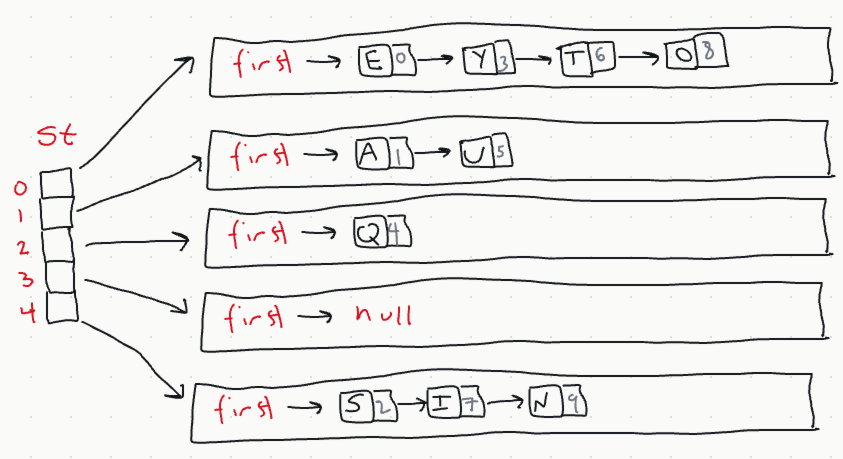
\includegraphics[width=0.7\textwidth]{exercise-01}
			\caption{Separate Chaining Hash Table from keys \texttt{E A S Y Q U T I O N}.}
			\label{fig:ex-01}
		\end{figure}
	\end{sol}
	
	\pagebreak
	\printbibliography
\end{document}